\begin{comment}

\section{ER Systems.}
\label{sec:erSystems}

Stanford NER: Consultar \cite{plu2015hybrid}

MITIE

Twitter_nlp

TwitIE

\end{comment}

\section{ED Systems.}
\label{sec:edSystems}

{\color{red} Creo que será mejor cambiar la subdivisión a Scoring y ML, en lugar de BoW, Graphs y ML. Los dos primeros se incluirían en Scoring. Decidir cuando estén todas las herramientas.}

\newcommand{\newRow}[7]{
	#1 & #2 & #3 & #4 & #5 & #6 & #7 \\
}

\newcommand{\localTechniques}[5]{
	#1 & #2 & #3 & #4 & #5
}

\newcommand{\collectiveTechniques}[6]{
	#1 & #2 & #3 & #4 & #5 & #6
}

\begin{table}[!ht]
\begin{tabularx}{\textwidth}{Xcllllccccc}
	\multicolumn{11}{c}{\textbf{Local methods}} \\
	\hline
	\multirow{2}{*}{Name} & \multirow{2}{*}{Year} & \multirow{2}{*}{Text type} & \multirow{2}{*}{KB} & \multirow{2}{*}{Approach} & \multirow{2}{*}{Has NIL} & \multicolumn{5}{c}{Techniques} \\
	\cline{7-11}\\[-8pt]
	&&&&&& T1 & T2 & T3 & T4 & T5 \\
	\hline\\[-8pt]
	
	\newRow{Mihalcea and Csomai}{2007}
	{General, HTML}
	{Wikipedia}
	{Bag of words}
	{No}
	{\localTechniques{x}{}{}{x}{}}

	\hline
\end{tabularx}

\caption{Summary of local systems.}
\end{table}

\begin{table}[!ht]
\begin{tabularx}{\textwidth}{Xcllllcccccc}
	\multicolumn{11}{c}{\textbf{Collective methods}} \\
	\hline
	\multirow{2}{*}{Name} & \multirow{2}{*}{Year} & \multirow{2}{*}{Text type} & \multirow{2}{*}{KB} & \multirow{2}{*}{Approach} & \multirow{2}{*}{Has NIL} & \multicolumn{6}{c}{Techniques} \\
	\cline{7-12}\\[-8pt]
	&&&&&& T1 & T2 & T3 & T4 & T5 & T6 \\
	\hline\\[-8pt]
	
	\newRow{Mihalcea and Csomai}
	{2007}
	{General, HTML}
	{Wikipedia}
	{Bag of words}
	{No}
	{\collectiveTechniques{x}{x}{}{x}{}{x}}
	
	\hline
\end{tabularx}

\caption{Summary of collective systems.}
\end{table}

Factores para tabla:

\begin{multicols}{3}
\begin{enumerate}
	\item Name
	\item Year
	\item Reference
	\item Knowledge base
	\item Text type
	\item Approach (scoring, graphs, ML)
	\item Techniques (columns and \tick)
	\item Has NIL
	\item ¿Only named?
	\item ¿Domain selection?
\end{enumerate}
\end{multicols}

\begin{figure}[!ht]
	\centering
	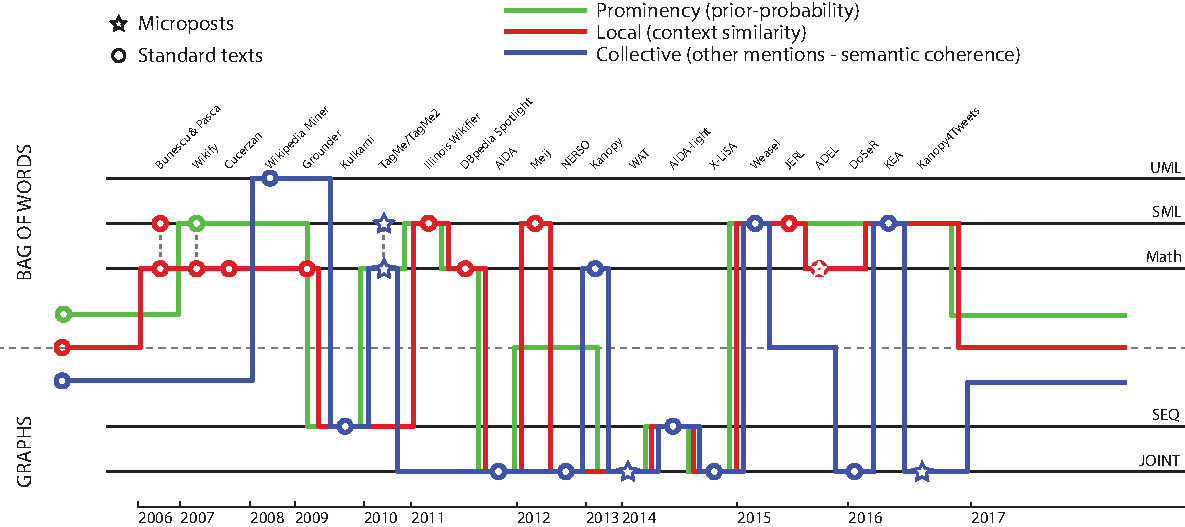
\includegraphics[width=\textwidth]{toolRoadMap}
\end{figure}

\subsection{Prominence Methods.}

To the best of our knowledge, there is not any system that only relies on statistical information or prior probability. A system with this characteristics would be so simple and limited in their effectiveness that there is not much to research in this direction. However, a prominence factor is used in almost every NERD systems, as it favours most frequent entities over more obscure ones with a simple to work with magnitude.

%\subsubsection{Bag-of-words Systems.}

%\subsubsection{Graph-based Systems.}

\subsection{Local Methods.}

\subsubsection{Bag-of-words Systems.}~

\medskip

\cite{mihalcea2007} introduce the term of \emph{Wikification} of a text, that is, convert every relevant mention in a text into a hyperlink to a resource that describes the represented entity. In this case, the resources are Wikipedia articles. This works are based on word sense disambiguation and keyword extraction, so the general approach and many techniques are inherited from these sciences.

This approach is divided in the traditional three steps: pre-processing, keyword extraction (i.e. entity recognition) and word sense disambiguation (i.e. entity linking). ER is performed by querying the surface form dictionary with all the n-grams in the text and then raking it based in up to three different measures. Then, the top \emph{k} candidate mentions are selected as relevant terms, where \textit{k} is determined based on the link frequency in Wikipedia (around 6\% as pointed in the paper). To perform the disambiguation they combine two algorithms in an agreement schema: an annotation is correct when both algorithms say so. First one leverages the similarity between the mention context and the Wikipedia article. The second one uses a machine learning approach based on a Naive Bayes classifier, which uses the context of the mention, its POS tags and some frequent words from the input text as features for the decision making.

\medskip

\cite{cucerzan2007}'s approach leverages contextual information to make the decisions during the disambiguation task. He uses Wikipedia to generate the information about entities, surface forms and categories (these extracted from list pages), although the scope of the system is restricted to named entities only. Recognition of entities is performed with a recognized that uses simple mechanisms like capitalization rules and statistical information to detect the boundaries of the mentions. Disambiguation is accomplished by querying the surface form dictionary to get the candidate entities that could be represented by the gathered mentions. Then, for each mention and candidate entity a vector is generated, which contains contextual and category information about them. Each mention-entity pair is then scored with the scalar product of both vectors, so the pair that maximizes this value (which is not normalized to take in account the prominence of each candidate) is taken as the correct one.

\medskip

\cite{fader2009} give a greater weight to the prominence factor in the ERD process. As pointed before, prominence information by itself is not very reliable, as it has an implicit and unavoidable error margin. However, this error is smaller when an entity is much more probable than the rest, which a frequent fact, so it may be useful to leverage this factor in a general scenario. Moreover, this is how the human mind uses to work.

The authors combine the prominence factor with a contextual similarity measure to perform the disambiguations task. First one is obtained based on the number of wikilinks that point to an article, so the more an article is referenced, the higher will be its prominence value. The contextual comparison is performed through the cosine similarity function (see \autoref{sec:techniques:context}) between the whole input text and the article of the entity. The final score for each mention-candidate entity pair is the product of these values.

\medskip

DBpedia Spotlight (\cite{mendes2011}) is one of the most prominent projects in ERD development. DBpedia Spotlight finds and annotates mentions with DBpedia resources, which is used as the underlying knowledge base. The well-structured DBpedia Ontology let the user to restrict the process to a certain domain, which improves the precision of the system in specific application environments.

DBpedia Spotlight performs both recognition and disambiguation. First, exact string matching is used to look for surface forms in the input text. These surface forms are obtained from the ID labels, redirection pages and disambiguation pages in DBpedia, as well as which resources they link. Then, for each surface form all the candidate entities (and their prior probability for the corresponding mention) are extracted and considered during the disambiguation phase.

Each candidate is represented as a word vector containing all the paragraphs that contain a wikilink to the Wikipedia article that describes the entity. Each word is then weighed with the product of its TF, or term frequency within the resource, and its ICF, or inverse candidate frequency. ICF is a novel measure that indicates the discriminative power of a word: the more resources it is related with, the less discriminative power it has. The context of the mention is represented in a similar manner, so the cosine similarity measure (see \autoref{sec:techniques:context}) can be applied to score the contextual coherence between a mention and each of its candidate entities. Finally, the candidate with the highest score is used to annotate the mention, although we can set a minimum confidence score so only annotations with a higher score than this threshold are performed.

The system was further developed and extended to a multilingual approach in \cite{daiber2013}. This update introduces alternative methods to work with the data in a language-independent manner. During the recognition step, combinations of tokens that form known surface forms are generated and looked for them in the input text, while in the language-dependent implementation some linguistic resources are leveraged, e.g. capitalization or noun phrase detection by POS tagging the input text. Candidate generation remains the same.

Disambiguation is performed using the generative probabilistic model proposed in \cite{han2011generative}. It combines three parameters to calculate a score for each candidate entity: the prior probability of the entity (number of incoming wikilinks), the probability of that the surface form represents that entity (number of wikilinks with the surface form as anchor text that link the entity), and the score of the context of the entity. Then, the candidate with the highest score is selected for each mention.

\medskip

\cite{caliano2016} focus on linking entities in microposts. They rely on a third party NER system to extract all the mentions from the input text, T-NER (see \autoref{sec:erSystems}), but only after pre-processing it accordingly to the nature of this kind of texts. This way, some special characters are removed, like the `\#' or `@' that are common in tweets, and some segments, like hashtags, are transformed into more standardized phrases. 

Then, they obtain, for each mention, the possible resources from DBpedia that could represent the correct annotation. These resources are ranked in function of a \emph{knowledge base score}, so only the top results are retrieved as candidates for a mention. This score is calculated based on three factors:
%
\begin{enumerate*}
\item similarity between mention and the \texttt{rdfs:label} field of the candidate resource (Jaro-Winkler distance, see \autoref{sec:techniques:context}),
\item cosine similarity between the mention context and the description (abstract) of the candidate resource, and
\item popularity measure of the candidate in the knowledge base (Page Rank).
\end{enumerate*} 
%
Finally, the candidate that reaches the highest score is used to annotate the mention.

\begin{comment}

\noindent\rule{\linewidth}{1px}

\tick\nuevaHerramienta{\cite{mihalcea2007} Wikify}
{2007}
{Wikipedia}
{Prominence + Local}
{N-grams}
{Dictionary (exact matching) + Refinement with three measures: TF-IDF, $X^2$ independence test and keyphraseness (prominence)}
{Two methods: Overlapping between contexts; and SML classifier (Naive Bayes) based on prominence.}


\tick\nuevaHerramienta{\cite{cucerzan2007} Cucerzan}
{2007}
{Wikipedia}
{Joint (Local)}
{Capitalization analysis}
{Capitalization rules + Dictionary. Classification in Person, Location, Organization or Miscellaneous. Candidate detection with partial matching.}
{For each possible combination of entity annotations, overlapping between document vector (which aggregates all the contexts and categories of the detected surface forms) and entity vector (which aggregates the Wikipedia contextual information and categories of the selected candidates)}

\tick\nuevaHerramienta{\cite{fader2009} \textsc{grounder}}
{2009}
{Wikipedia}
{Prominence + Local}
{Unknown}
{Unknown (probably dictionary with surface forms taken from Wikipedia)}
{Prominence + Cosine Similarity Function between context of the mention and each candidate entity's context info (combined through Bayes' theorem)}

\tick\nuevaHerramienta{\cite{mendes2011,daiber2013} DBpedia Spotlight}
{2011}
{DBpedia}
{Prominence + Local}
{LingPipe Exact Dictionary-Based Chunker using the surface form catalog}
{Dictionary}
{Cosine Similarity Function between contexts + Prominence + Inverse Candidate Frequency}

\tick\nuevaHerramienta{\cite{caliano2016} UniMiB}
{2016}
{DBpedia}
{Prominence + Local (Microposts)}
{T-NER (Ritter et al.)}
{T-NER (Ritter et al.): CRF}
{Scoring based on popularity of each entity and lexical similarity (both contextual and from the mention)}

\noindent\rule{\linewidth}{1px}

\end{comment}

\subsubsection{Graph-based Systems.}~


\subsubsection{Machine Learning.}~

\cite{bunescu2006} may be considered the first NERD system. This work lays down the foundations for the standard pipeline of mention detection, candidate generation and entity disambiguation, as well as the surface form dictionary linked to the entity catalogue, both generated based on Wikipedia. However, it is restricted to named entities only, that is, those with proper names.

Their approach treat disambiguation as a ranking problem. To solve it, they propose a supervised machine learning approach using support vector machines (see \autoref{sec:techniques:ml}). They use the Wikipedia itself to build many training sets, where the wikilinks in the articles are positive examples, and the candidates that are not linked by them are negative examples. As features for the score calculation, they use cosine similarity, to measure the correlation between each mention's context and the article of each candidate entity, and the Wikipedia taxonomy, to determine the degree of semantic coherence between a mention and the super-categories of each candidate entity. At last, they implement a mechanism to detect and report mentions that do not represent any entity in Wikipedia, which consists on a minimum threshold for the score of the best candidate.

\medskip

\cite{meij2012} was one of the first systems at taking the ERD pipeline to microposts, particularly Twitter. However, this is done at tweet-level, not word-level, so it could be considered as text classification with concepts instead of semantic classes. This system consider as an input every n-gram found in a tweet, so a ranked list of candidate entities is obtained for each one of these candidate mentions in an effort to maximize the recall. To this end they test up to six approaches, being the optimal the CMNS method, proposed by the authors. CMNS measures the frequency with which a n-gram (that is, a surface form) is used as anchor to link a certain concept in Wikipedia, so it is a plain prominence feature. However, it behaves well and provides good results in terms of significance and performance.

For the disambiguation step they implement a supervised machine learning approach with Random Forest as the learning algorithm (see \autoref{sec:techniques:ml}). The training set consists on a number of labeled examples where concepts are annotated with a set of relevant articles. Combining an extensive set of features, the set of candidate concepts that were gathered during the previous phase is re-ranked to select the most relevant ones for the whole tweet.

\cite{yamada2015} take Meij's work as a starting point, and also specialize in microposts. They implement machine learning for the whole ED process, although they use more traditional methods for the ER phase. For this task, they use a dictionary built from Wikipedia data (titles of the articles, redirection and disambiguation pages, and wikilinks' anchor text). This dictionary is queried with all the n-grams from the tokenized tweet through multiple criteria, including exact or approximate match and acronym search.

The resulting mentions and candidate entities are used as input for a supervised model following \cite{meij2012}, although they add  three new features: 
%
\begin{enumerate*}
\item contextual information using word embeddings,
\item temporal popularity knowledge of an entity using the tweet's date and the Wikipedia page view data, and
\item string similarity measure between the mention and the title of the article.
\end{enumerate*}

This system also introduces three novelties: an overlapping resolution mechanism, a NIL mention detection system and the prediction of the mentions' type. The overlapping resolution mechanism is applied after the disambiguation phase, and it analyses if a mention is already contained in a previous one, and only keeps the mention with the greater score and discards the remaining ones. On the other hand, NIL detection is tackled as a classification problem where random forest is used again, but with different features. Finally, mention typing is applied over both NIL and non-NIL mentions using two different machine learning models, which use logitic regression and random forest as learning algorithms, respectively. 

\cite{greenfield2016}'s approach builds over the previous one, \cite{yamada2015}, although this uses DBpedia instead of Wikipedia as the knowledge base. However, the main difference is that they propose an inverse approach for the annotation of entities in tweets: for each entity in the knowledge base, they look for each one of their surface forms in the input tweet. Then, a list of mention candidates is generated for every entity that may appear in the text.

This let us to easily define an specific domain, as well as maintaining their possible surface forms (which could include misspelled forms or frequent variations in this kind of media), because of the top-down approach. Correct spots are determined through machine learning with random forest, same as the works this bases on, but with a more restricted set of features. They experimented with AIDA (\cite{yosef2011}) as their ED engine, but it provided very poor performance when dealing with non-person entities. On the other hand, ER is accomplished through a voting system between multiple recognitions systems.

\medskip

\cite{zheng2012} use Freebase as knowledge base for their proposal. The argument given is that it is richer in entities than Wikipedia. However, it lacks contextual information of them, which is compensated with two features of Freebase: its vast amount of recognized surface forms for its entities, and the rich taxonomy it owns, which make Freebase a more solid information source for both humans and machines.

The authors propose an iterative procedure, where the unambiguous mentions are annotated and later used to disambiguate the remaining mentions. {\color{red}[COMPLETAR]}

\medskip

The proposal in \cite{rao2013} is an EL only system, delegating in third-party tools the recognition of entities in a text. They use Wikipedia as their knowledge base, but try to define a non Wikipedia specific approach in terms of what resources they use from the knowledge base. Their linking pipeline is as follows: first, they gather candidate entities for the input mentions by a string matching method procedure that combines exact matching, overlapping and different similarity measures between each mention and the entries in the surface form dictionary.

After the candidates are identified, they use a supervised machine learning ranker to determine the optimal candidate entity for each mention. They use support vector machines (see \autoref{sec:techniques:ml}) with maximum margin; that is, a candidate entity is selected if it gets the greatest score over every other candidate by a prefixed margin. This should also let us control the confidence of the assignation by tweaking the imposed margin. To make a decision, the system uses a plethora of features about entities, surface forms, Wikipedia features (which would not be present in case of using other knowledge base), etcetera. A novel and interesting magnitude that they take in account is the rank of the Wikipedia article in a Google search as a measure of the prominence or popularity of the entity.

\medskip

\cite{durrett2014}'s proposal uses conditional random fields (see \autoref{sec:techniques:ml}) to tackle the ERD task. They implement entity typing (entity recognition) and coreference detection (that is, detection and clustering of the mentions to a same entity) in conjunction with entity linking in an unique joint pipeline, so every operation can support the remaining to lead to a better result.

For every proposed mention, a list of candidate entities is generated by what is called a \emph{query}: they use not only the whole mention, but all its prefixes to query the surface form dictionary (which is generated based on Wikipedia). Coreference helps ER by ensuring the consistency between the semantic types of similar mentions -- making them to have same POS tags --, but is quite less useful in combination with EL, as the same mention can refer to different entities each time. On the other hand, the combination of ER and EL in a joint task has been pointed by other authors (\cite{luo2015}, \cite{nguyen2016}). There, entity assignments from EL step may provide some information about semantic types thanks to the semantic categories the entities belong to, and vice versa. {\color{red}[REVISAR: ML durillo]}

\medskip

\cite{perera2016} focus an uncommon aspect of the ERD problem: implicit mentions linking. In microposts, the kind of texts this work is oriented to, it is frequent to elide the name of the entity they talk about for the sake of brevity. In these cases, there are no surface forms that could be recognized in the text, so the recall drops to the ground, leading to a poor final result. To overcome from this circumstance, they leverage the contextual information (the tweets that are simultaneously published), temporal salience and factual knowledge.

Contextual information comes from the tweets that are published in a short window of time around the tweet we want to annotate. These tweets may contain not only explicit mentions that may be easily detected and resolved to an entity, but also frequent words or phrases that may be used instead of the implicit mention. Temporal salience is a prominence measure based on the number of views of the Wikipedia article of an entity in the last 30 days. Factual knowledge consists on affirmations and semantic relations with other entities that could be explicit in the tweet. All this information is joined in an Entity Model Network (EMN), whose construction is detailed in the paper.

For the ERD task, the system first generates a reduced model based on the explicit mentions in the tweet. To this end, it queries a surface form dictionary built based on Wikipedia and saves them as ``tweet clues'' to get a graph of candidate entities. This sub-model is used as input for a ranking machine learning model, a SVM, based on pairwise approach; that is, it takes all candidate entity-mention pairs and ranks them in function of which pair is better. To this end, it takes into account the temporal salience and the cosine similarity between the tweet and the entity features (titles of the entities that are connected with the candidate) represented as a vector.

\begin{comment}

\noindent\rule{\linewidth}{1px}

\tick\nuevaHerramienta{\cite{bunescu2006} Bunescu and Pasca}{2006}
{Wikipedia}
{Local}
{Unknown}
{Dictionary (exact matching)}
{Cosine Similarity Function between context of the mention and each candidate entity's context info + SML: SVM Classifier (Naive Bayes) for Wikipedia category correlation}

\nuevaHerramienta{Illinois Wikifier}
{2011}
{Wikipedia}
{Prominence + Local}
{Unknown}
{Manual localization + Dictionary}
{SML Ranking SVM with multiple features: Cosine Similarity Function between contexts, PMI, NGD...}

\tick\nuevaHerramienta{\cite{meij2012} Meij}
{2012}
{Wikipedia}
{Local}
{N-grams}
{Dictionary (exact matching), contextual information or another systems that do NER operations}
{SML (Random Forests Algorithm)}

\nuevaHerramienta{\cite{zheng2012} Zheng et al.}
{2012}
{Freebase}
{Local}
{-}
{-}
{ML. NED only: Semi-supervised, two models: generative and discriminative}

\tick\nuevaHerramienta{\cite{rao2013} Rao et al.}
{2013}
{Wikipedia}
{Prominence + Local}
{-}
{-}
{Supervised ML.}

\tick\nuevaHerramienta{\cite{durrett2014} Durret and Klein}
{2014}
{Wikipedia}
{Local}
{N-grams}
{Grammatical features for the SCRF}
{Structured CRF}

\tick\nuevaHerramienta{\cite{yamada2015} Yamada et al.}
{2015}
{Wikipedia}
{Prominence + Local (Microposts)}
{-}
{Dictionary}
{Random Forest}

\tick\nuevaHerramienta{\cite{greenfield2016} Greenfield et al.}
{2016}
{DBpedia + YAGO}
{Prominence + Local (Microposts)}
{-}
{Dictionary}
{Random Forest}

\tick\nuevaHerramienta{\cite{perera2016} Perera et al.}
{2016}
{DBpedia}
{Prominence + Local (Microposts)}
{-}
{Based on contemporary tweets: they identify the explicit entities and take them as candidates for the implicit entities.}
{Focused on implicit entities (IEL). SVM.}

\noindent\rule{\linewidth}{1px}

\end{comment}

%%%%%%%%%%%%%%%%%%%%%%%%%%%%%%%%%%%%%%%%%%%%%%%%%%%%%%%%%%%%%%%%%%%%%%%%%%%%%%%%%%%%%%%%%%%%
%%%%%%%%%%%%%%%%%%%%%%%%%%%%%%%%%%%%%%%%%%%%%%%%%%%%%%%%%%%%%%%%%%%%%%%%%%%%%%%%%%%%%%%%%%%%
%%%%%%%%%%%%%%%%%%%%%%%%%%%%%%%%%%%%%%%%%%%%%%%%%%%%%%%%%%%%%%%%%%%%%%%%%%%%%%%%%%%%%%%%%%%%

\subsection{Collective Methods.}

Collective methods have been an interesting approach since the early days of NERD, but the first proposals were known for its high computational cost. In consequence, most of the systems that implement collective methods introduce many approximations to alleviate this problem, although the computational exigence of the process has moved from the complexity of the calculations -- as the processors' power has largely increased since 2006 and they can tackle harder problems in less time --, to the scalability of the process.

The introduction of graphs as a tool for solving this problem entailed a great impulse for the collective methods. Graphs not only let us model the needed information in an intuitive manner -- as the entity-relationship model is highly similar to the classic node-edge graph, directed or not --, but they also provides a set of algorithms and procedures that are common in graphical processing.

\subsubsection{Bag-of-words Systems.}~

\textsc{TagMe} \cite{ferragina2010} is one of the most successful systems that carries out the ERD-in-microposts problem. Its main goal is to provide with a system that is capable of annotate short texts --in this case, tweets-- with Wikipedia articles on-the-fly, that is, in almost real time. As we pointed before, the generation speed of microposts is very high, so a very agile and light processing is required to annotate them as they are generated.

Both the surface forms and entities are gathered from Wikipedia. For each surface form, they register the proportion of times it is used as anchor text in a wikilink (\emph{link probability}); and the probability of it linking each one of its possible candidate entities (commonness or prior probability). They do not indicate any procedures for the recognition, so we assume that mentions should be tagged in the input text.  Candidate entities are generated by querying the surface form dictionary and retrieving all the possible senses for each one of them. Then, this candidate senses are scored and ranked to determine the optimal one. 

The scores are generated through a voting scheme: for each candidate sense, all the candidates of the remainder mentions are analysed to measure the relatedness between them (in case a mention have more than one candidate, they calculate the average relatedness score for all its candidates, which are pondered with their prior probability) and said candidate sense. The proposed relatedness measure is Milne and Witten's function (see \autoref{sec:techniques:semantic}).
\begin{comment}
, the formula being:
%
\begin{equation}
\mathrm{vote}_b(p_a) = \frac{\sum_{p_b \in P_g(b)}{} rel(p_b,p_a)\cdot P_r(p_b|b)}{|P_g(b)|}
\end{equation}
\end{comment}

To this end, they propose two algorithms:
%
\begin{enumerate}
	\item Disambiguation by classifier: A classifier that combines commonness and the relatedness score of each candidate to generate a ``probability of correct disambiguation'', and assigns that with the highest score.
	\item Disambiguation by threshold: This algorithm selects the top \textit{k} candidates in base to their relatedness score and recalculates its score after discarding the remainder senses. Then the one with the highest score is used to annotate the mention.
\end{enumerate}

Finally, a pruning phase is performed over the result set to discard irrelevant mentions. For each mention, a value is generated using two parameters: the link probability of the mention, and the coherence between the annotated entity and the entities used for the remainder of the mentions. The calculation of this value can be carried out with an arithmetical combination of both factors, or through a machine learning classifier (SVM and C4.5 are mentioned as possibilities). This way, all the mentions that are not coherent with the rest of the text are deleted from the final result.

\textsc{TagMe} was updated and received its version 2.0 in \cite{ferragina2012}. There they describe a pre-processing and recognition algorithm, which the past version lacked, that consists on extracting a set of n-grams from the text and removing those that do not bring any result when querying the surface form dictionary. Then, overlapping between mentions is solved by keeping the longer ones, unless the shorter ones has a much bigger link probability. 

The disambiguation phase remains unchanged, including both disambiguation algorithms, but they add two thresholds for the values of link probability and commonness of the candidate mentions and candidate entities, respectively, to tune the process in order to improve the accuracy or the efficiency with a minimal trade off with the recall.

\medskip

\cite{scaiella2014} propose DataTXT, presented as the evolution of \textsc{TagMe}. DataTXT keeps the general pipeline and algorithms of \textsc{TagMe}, but adds some new features and improvements. For instance, during the disambiguation step a new parameter is introduced to weigh the influence of context and commonness (prior probability). The rest of changes are different adaptations to the requisites of the Microposts 2014 challenge, to which DataTXT was one of its contestants.

\medskip

\cite{hulpus2013} describe Kanopy, an ERD system that leverages the DBpedia's semantic network to generate additional wealth from natural language texts beyond the mere entity linking. Kanopy generates a graph that semantically describes the whole input text, and provides with a semantic contextualization of the recognized concepts, as well as a list of the most relevant topics in the text. First, it extracts the relevant phrases from the text, i.e. noun phrases through Stanford CoreNLP. Then, it cluster them depending on the topics behind these phrases using diverse techniques.

The ERD task is performed using WSD and Eigenvalues (see \autoref{sec:techniques:semantic}), described by the authors in \cite{hulpus2012}. From the set of DBpedia resources used to annotate the mentions, Kanopy build a graph by expanding two levels an initial graph that contains them all. This graph is used to generate the most relevant concepts by performing a ranking algorithm to measure the semantic centrality of each node that corresponds with an annotated resource.

\medskip

\cite{liu2013} tackle the entity linking in short texts by leveraging three types of coherence -- mention-entity, entity-entity and mention-mention -- to provide result that maximizes the coherence between each one of the annotations, following the hypothesis that all entities in a text should be related to some extent. This systems only performs ED, so the input text should already have all the mentions tagged manually or by using another ER system.

Candidate entity generation is performed by looking at the surface form dictionary. For each candidate entity, a score is generated using three parameters:
%
\begin{enumerate}
\item Mention-entity similarity: Many features are used to model this score, which include prior probability over the set of Wikipedia's wikilinks, the proportion of words that are common to both the tweet and the Wikipedia article, and some binary factors that indicates the edit distance similarity, and whether the mention contains the title of the entity, or the title of the entity contains the mention.
\item Entity-entity similarity: In order to obtain this value, authors use the Milne and Witten formula (see \autoref{sec:techniques:semantic}).
\item Mention-mention similarity: Some string comparisons are performed over each pair of mentions, e.g. cosine similarity or the edit distance between them; and two contextual features that point whether both mentions belongs to tweets from the same account, and whether both mentions contain a common hashtag.
\end{enumerate}
%
These values are pondered with some additional parameters that do not depend on the input text, but are prefixed or obtained from a training set instead. The set of entities that maximize the sum of all its values is selected as the correct assignations for the input set of mentions.

\medskip

\cite{sodergren2017}'s proposal belongs to the multilingual approach for ERD. This system leverages Wikipedia to obtain entities and surface forms, but also uses Wikidata as the central entity repository in order to get access to the structured data it contains, like dates, and its multilingual information. Additionally, some features are gathered to use them during the annotation process: prior probability of each entity with respect to a mention, an approximation of the ambiguity of each mention, if there are proper names or stopwords in a mention, etcetera.

Mentions are spotted by looking for any known surface forms from the dictionary in the input text. The results are pruned by applying some simple manually-written rules to remove irrelevant mentions in order to improve the precision, but trying to without harming the recall. Some examples are capitalization analysis or a threshold for the link probability of a mention (the frequency with which it acts as a wikilink over all its appearances in Wikipedia).

For the disambiguation step they apply the Page Rank algorithm up to three times over an undirected graph where each mention-entity pair is included as a node, and the nodes are linked when %
\begin{enumerate*}
\item the article of one entity has a wikilink to the article of another entity in the graph, or
\item two links to both entities are found in a same paragraph in Wikipedia.
\end{enumerate*}
%
After this step, all the nodes should have a score. Then, a weighted category graph -- generated by relating each article in Wikipedia with its main categories along all its versions in other languages -- is used to determine the coherence between each candidate article and the set of categories of the core entities in the text, i.e. those that do not present ambiguity.The highest scored entities for each mention are used to perform the annotation. 

{\color{red} [REVISAR: Confuso. Ver \cite{eckhardt2014}, en el que se basan estos señores.]}

\begin{comment}

\noindent\rule{\linewidth}{1px}

\tick\nuevaHerramienta{\cite{ferragina2010,ferragina2012} TagMe/TagMe2}
{2010}
{Wikipedia}
{Prominence + Collective (Microposts)}
{N-grams}
{Dictionary}
{Prominence + Collective agreement between the candidate entities (M\&W). This values are combined through one out of two methods: Disambiguation by classifier (ML), or Disambiguation by Threshold.}

\tick\nuevaHerramienta{\cite{hulpus2013} Kanopy}
{2013}
{DBpedia}
{Collective}
{Stanford CoreNLP}
{Stanford CoreNLP NER + Noun phrase clustering phase}
{Word Sense Disambiguation usin eigenvalues}

\tick\nuevaHerramienta{\cite{liu2013} Liu et al.}
{2013}
{Wikipedia}
{Prominence + Local + Collective (Microposts)}
{-}
{-}
{Ranking with prior, context similarity, co-ocurrence of mentions and M\&W among others.}

\tick\nuevaHerramienta{\cite{scaiella2014} DataTXT (evolution of TagMe)}
{2014}
{Wikipedia}
{Collective (Microposts)}
{-}
{Dictionary}
{Scoring}

\tick\nuevaHerramienta{\cite{sodergren2017} HERD}
{2017}
{Wikipedia + Wikidata}
{Local + Collective (Multilingual)}
{-}
{Dictionary: Solr Text Tagger + Lucene}
{Scoring: PageRank + Category coherence}

\noindent\rule{\linewidth}{1px}

\end{comment}

\subsubsection{Graph-based Systems.}~

\cite{kulkarni2009} introduce the graphical approach into the ERD task. Apart from providing with a somewhat intuitive representation of mentions and entities, it brings us the possibility of measuring the semantic coherence between the candidate entities by jointly considering them in the disambiguation problem.

This system builds over Wikipedia as the source for the entity catalogue and the list of surface forms for each entity. Mentions are extracted through partial matching between segments in the input text and a surface form from the dictionary. Four pieces of information are gathered for each entity: both the introduction paragraph and the full Wikipedia article, the set of all anchor texts used to link this article, and a context for each one of these anchors. Authors use this data to measure the contextual similarity between a mention and each of its candidate senses. Both contexts are compared through different measures to improve the confidence. A prior probability factor is also considered based on the frequency with which a surface form is used in Wikipedia to link a specific article.

A novel factor in this work is the relatedness degree between entities, whose calculation relies on Milne and Witten's WLM to determine the pair-wise semantic coherence. Then, the challenge is to find the assignment that maximizes the combination of contextual and semantic coherence. Here lies the downside of the graphical approach: the computational cost may be very high. To this end, authors propose two approximations (a LP rounding approach and a hill-climbing algorithm), which are compared with a context-only approach as the baseline. Although both algorithms brings better results than the baseline, there is not a clear winner: first one provides with better results, but the latter is more lightweight. This is an habitual trade-off in this kind of environments.

\medskip

\cite{yosef2011} present AIDA, one of the most prominent proposals in ERD development. AIDA is characterized by its powerful, yet computationally heavy, recognition and disambiguation pipeline, which brings accurate results by making use of a complex graphical model. Its graphical approach allows to use both statistical, contextual and semantic coherence data to find the densest subgraph that contains the optimal combination of annotations for the observed mentions.

AIDA's pipeline is further explained in \cite{hoffart2011}. First, mentions are discovered by using Stanford NER Tagger, which yields a high precision, high recall input for the candidate generation step. Candidates are obtained from YAGO, a knowledge base that is developed by the authors of AIDA, by looking for the observed mentions among the surface forms that are stored in YAGO. Then, each candidate is scored with a function that combines prior probability of each candidate given the found surface form, the similarity between the mention's context and the stored contextual information of the candidate entity, and the semantic coherence between all the candidates. These parameters are weighed accordingly to the values obtained from a SVM classifier.

To tackle this optimization problem, authors choose to implement a undirected graph-based method. Both mentions and candidate entities are included as nodes. Then, two types of edges are created: mention-entity edges, and entity-entity edges. Then, mention-entity edges are weighed with the similarity between the mention and the entity based on their context: the input text for the mention, a set of key phrases for the entity (e.g. titles and anchor texts from Wikipedia). Entity-entity edges are weighed using Milne and Witten's WLM.

Once the graph is constructed, the optimal combination of annotations that maximizes the objective function must be found. However, this problem is NP-hard and must be tackled by using an approximation. First, a distance to its mention node is calculated for every entity node, so only the closest $n$ nodes are kept and the remainder are removed from the graph. Then, authors apply a progressive pruning of the least significant candidate for the set of mentions, unless it is the last candidate for a mention (\emph{taboo node}). After each deletion, values from all the nodes are updated. When each mention has only one candidate entity, that graph contains the optimal mention-entity assignation for the input set of mentions. An alternative local-search approach is also proposed, where candidate entities for each mentions are randomly selected by using its weights as a ``jumping probability'', and repeating this process a fixed number of times, although this method ignores coherence between entities.

\medskip

\cite{han2011} go beyond \cite{kulkarni2009} and propose a global interdependence model in opposition to their pair-wise coherence approach. To this end, they construct a graph, the Referent Graph, that aims to capture both the similarity between a mention and a candidate entity and the coherence in the set of all candidate entities for every mention in an input text. Mention nodes are connected with their candidate entity nodes, and then each pair of entity nodes are linked with a undirected, weighed edge if there exists a semantic relation between them.

Mention-entity correspondence degree is measured by analysing the co-occurrence of words in their respective contexts, represented by two vectors where each word is weighted with its TFIDF score. The context information for each entity consists exclusively on its Wikipedia article. On the other hand, semantic relation between entities is scored with Milne and Witten's WLM.

The disambiguation model can be presented as a random walk with restart on graphs approach. First, each candidate is scored based on its \emph{prior importance}, i.e. its TFIDF score, as a form of relative pre-ranking of the candidates. These values will be used as the \emph{initial evidence} of the correct annotation for the input mention set. A matrix is constructed with the factors that weigh each pair of candidate entities in the referent graph, where each value can be seen as the hop-probability between two nodes. If a node has not outgoing relations, i.e. is not connected to any other candidate entity, a \emph{restart} is performed to avoid to interrupt the evidence propagation and its disappearing at that node. This restart consists on transferring a part of the propagating evidence to the initial evidence after every step. This way, initial evidence is propagated though the set of candidates, so a accumulated value is obtained for each candidate entity. Then, the candidate with the highest score is used to annotate each one of the input mentions.

\medskip

\cite{hachey2011} bring a WSD approach to entity linking. They propose a theoretical graph with all the articles and categories from Wikipedia by leveraging its wikilinks' structure. First, candidates are generated by querying the index of entities, that is, looking for Wikipedia titles that match each mention from the input text. Then, a subgraph that contains all the candidate entities, as well as all the intermediate nodes that form paths between the said nodes, is extracted from the global graph. To keep the graph size under control, they impose a fixed maximum path length, which is set to 2 for entity nodes, and 3 for category nodes.

Then, the goal is to score each node in the graph to determine the optimal correspondence. They propose two graph measures to score each node: Degree centrality and Page Rank, which are combined with cosine similarity as contextual comparison measure. Degree centrality is the proportion of incoming edges of each node over the total of nodes minus one. Page Rank has its usual formulation. ({\color{red} Verificar.}) On the other hand, cosine similarity is calculated between the paragraph where the mention is, and the whole Wikipedia article that describes a candidate entity. The entity with the highest score is selected as the correct one for each mention.

\medskip

\cite{hakimov2012}'s NERSO, which stands for Named Entity Recognition Using Semantic Open Data, performs recognition and linking using DBpedia and a graphical approach. They use a centrality measurement algorithm to identify the correct entity for each one of the ambiguous mentions in an input text. First, they perform a spotting step, where a sliding window is applied on the input text in search of segments --sets of consecutive words-- that matches the titles of the DBpedia resources that form its surface form dictionary. This sliding window has a fixed initial length that is reduced if a segment does not correspond to any known surface form.

The graph is built using the {\smaller \texttt{dbont:wikiPageWikiLink}} from DBpedia, which are ultimately obtained from the wikilink set from Wikipedia. This originates a directed graph where all the candidate entities are represented as nodes, and the edges are created based on its links to other candidate entities in DBpedia. On this graph, they apply a centrality scored method where the score for each node is the number of reachable nodes from it --that is, the nodes to which there exists a path--, divided by the sum of the lengths of the shortest path to each one of them. The method that is used to determine these path's lengths is the Djikstra's algorithm.

This centrality score is combined with the number of incoming links, outgoing links and a factor that indicates the type of node to generate the final score. Then, the highest scoring candidate entity is assigned to each spotted mention.

\medskip

In \cite{hakimov2016}'s NERFGUN, authors take some ideas from previous works and expand them by looking at other proposals in the state of the art. They propose an undirected, probabilistic graphical approach which makes use of prominence, contextual similarity and semantic coherence between candidates during its pipeline. NERFGUN is a pure NED tool, thus it requires the mentions to be labeled before it starts the process. Candidates are retrieved by querying a dictionary, which is built using both DBpedia and Wikipedia, the first to gather named entities and some surface forms, and the latter to enrich the surface form dictionary using wikilinks' anchor texts.

NERFGUN uses factor graphs \cite{kschischang2001factorgraphs} to discover the correct disambiguation for the ambiguous input mentions. The factor graph includes both mentions and textual clues (tokens from the text for context comparison purposes) as \emph{observed variables}, and the set of entities that are referred to by these mentions as \emph{hidden variables}. The goal is to discover the optimal values for these hidden variables. To this end, they propose an optimization approach, where a random combination of candidate entities is taken as an initial step. Then, this assignation is iteratively transformed as follows: in each step, a set of combinations are generated by changing the current combination in only one mention annotation; from this set, the best combination is selected and passed to the next iteration. If no new combination is better than the current combination, it is kept. This procedure is repeated for a fixed number of iterations.

Generated combinations are scored by using a probability distribution function that comprises many factors:  entity frequency for a given mention, edit similarity --the Levenshtein distance between a mention and an entity--,  document similarity -- cosine similarity between the text and the initial paragraph of the Wikipedia article for an entity--, and two variants of Page Rank that aim to measure the popularity of the entity in Wikipedia and the semantic coherence between the entities used in a combination. After the iterative process, the resulting combination should be a correct assignation for the input mentions.

\medskip

\cite{nguyen2014} adapt the works in \cite{yosef2011} to a light-weightier pipeline to overcome its scalability issues, given the complexity of its computation process. They develop a thematic domain approach, which evaluates semantic coherence between entities by analysing its categories in a predefined ontology. Contextual information is introduced in the process by leveraging the fact of some mentions being unambiguous, so they constitute a solid ground to help to disambiguate the remaining mentions in a text.

AIDA-light starts with a text where the mentions has already been recognized and labelled. Then, a set of candidates is generated for each mention by querying a surface form dictionary. The exact matching method between mentions and surface forms is not indicated, but we can assume that is a partial or approximate matching. For each mention, two word sets are constructed for both the surrounding mentions and tokens for each mention. Then, unambiguous (``easy'') mentions are used to determine the domains which the input text belongs to, so these domains are added to the mention context of the remaining mentions. On the other hand, entities need to have a context set of words, which is filled with key tokens from their YAGO resources.

Disambiguation algorithm requires the combination of two dimensions:
%
\begin{itemize}
\item Mention-entity features: They include prior probability, mention-entity name similarity (based on the Jaccard coefficient between the mention and the entity name), mention-entity context similarity (using word overlapping between the token context and the key tokens of the entity), surrounding mention coherence (measured by the co-ocurrence in Wikipedia of the unambiguous entity and each one of the candidates), and the coherence between entities (by measuring the overlapping between their key tokens).
\item Domain-oriented features: They relate to the defined domain hierarchy, like the distance between the categories which two entities belong to.
\end{itemize}
%
Both sets of features join in an objective function, which lets us to score in a joint manner every candidate entity for the considered mention set. Disambiguation happens in two stages: first, only ``easy mentions'' are used as input on their own, excluding the remaining mentions (those with $\geq4$ candidates), and a graph is constructed using the top k entities, i.e. entities which bring the highest similarity value with the mention by using only its local features. Then, entities with the lowest entity and domain coherence are iteratively removed, recomputing the scores for the entities in each step. This is repeated until each mention has only one candidate entity. In the second stage, domains in the text are determined using the already disambiguated mentions. Then, the previous procedure is applied to the entities that remain ambiguous.

\medskip

\cite{usbeck2014agnostic,usbeck2014graph}'s approach, AGDISTIS, is a graph-based, knowledge base agnostic NED system. This fact requires a previous index creation step, where entities and their respective surface forms are gathered from the chosen knowledge base. Starting with a text where the mentions are already labelled, AGDISTIS generates candidates for each mention by using exact matching in the surface form index. Then, a two-step process is performed on the mentions: first, string normalization reduces each mention to its root, removing variations like plurals, genitives and time information; second, term expansion allows establishing relations between the mentions in text that point to the same entity. Reasoning behind this is that it is common that only the first reference to an entity is a complete surface form (e.g. name and last name: Bruce Springsteen), being the following mentions a substring of the first one (e.g. last name only: Springsteen). This is a simple implementation of \emph{coreference resolution} in a text. This way, the number of mentions that must be disambiguated can be drastically reduced. Finally, normalized mention and entity name are compared by using trigram similarity to measure their textual fitting to avoid noisy results by removing little relevant candidates.

To disambiguate between candidates, AGDISTIS builds a directed graph where candidates are included as nodes and edges are relations between pairs of entities, somehow defined in the underlying knowledge base (e.g. there exists a RDF triple that links them). Then, this graph is expanded in an iterative manner by adding the nodes from the KB that are related with the nodes already in the disambiguation graph. Lastly, HITS algorithm (see \autoref{sec:techniques:semantic}) is performed over this graph to rank the candidate nodes for each mention and to select the most authoritative one as the correct annotation.

\medskip

\cite{piccinno2014}'s WAT is a rework of \textsc{TagMe} in order to make its architecture modular and more efficient, and all its algorithms are revised. It keeps Wikipedia as its knowledge base, and all the structures that \textsc{TagMe} used to perform the ERD task. First, WAT analyses the input text looking for words or phrases that match one entry in the surface form dictionary. They also propose an optional binary SVM classifier that helps to determine if a mention is relevant or not.

Apart from the one that is implemented in \textsc{TagMe}, WAT propose a novel group of graphical algorithms, following the success of AIDA with these techniques. In it, both mentions and entities are represented as nodes, and between them there exist two types of edges: mention-entity, to describe the condition of candidate of the latter, and entity-entity, to indicate the fact that two entities are semantically related. The edges mention-entity can be weighted one out of three measures:
%
\begin{enumerate*}
	\item identity (weight always equal to 1),
	\item commonness (prior probability), or
	\item context similarity between the mention's context and the Wikipedia article.
\end{enumerate*} 
%
On the other hand, the edges entity-entity are weighted with the Milne and Witten's relatedness measure (see \autoref{sec:techniques:semantic}). They propose many algorithms to generate a score for each candidate entity, like Page Rank. For the pruning step, they train a SVM binary classifier to decide whether a mention is relevant or not, in addition to the pruner from \textsc{TagMe}.

\medskip

\cite{zhang2014} try to overcome the language problem of NERD by proposing a cross-lingual approach. Working in a multi-language environment greatly increases the amount of surface forms that need to be considered, so it could be difficult to determine which segments of a text are effectively mentions, and with which entity they should be annotated. A mono-lingual approach could also lead to miss many mentions that are expressed in a distinct language than the text's dominant one. Authors propose a model where information is represented in multiple languages based on multilingual Wikipedia and DBpedia \cite{zhang2014xlid}. For each entity in DBpedia, which is the grounding for their knowledge base, they gather all surface forms for that entity over the multiple versions of Wikipedia, as well as frequency statistics. Information in every language is then aligned to let an easy transposition from one language to the reference language.

Mentions are discovered through the analysis of the n-grams in an input text. In case of ambiguity a disambiguation algorithm is performed, which utilizes two kinds of features. These values will be introduced in a directed graph where mentions and candidate entities are included as nodes. Edges are introduced from mentions to entities, and between every pair of entities that are connected. First, mention-entity semantic similarity combine two different features: link probability as the prominence factor, and the value of cosine similarity between the mention's context and the entity's description vector in the reference language. The resulting value is used to weigh mention-entity edges. Second, entity-entity coherence is obtained by calculating the semantic relatedness between each pair of entities. To this end, authors use Normalized Google Distance over the wikilink structure from Wikipedia, an adaptation of Milne and Witten's approach.

On this graph, they perform a personalized Page Rank algorithm, which assigns a probability score to each entity node. Then, for each mention they assign the most probable entity to it.

\medskip

\cite{plu2015hybrid,plu2015revealing} propose a hybrid approach in three phases: recognition, linking and pruning. For the ER task, they rely on the Stanford NLP tools, more specifically the POS Tagger and the NER system in combination with two gazetteers for job names and nationalities (which help in the disambiguation step). The training details for these systems are detailed in the citation.

This system leverages both Wikipedia and DBpedia to generate an index of entities with a set of features, which will be used during the disambiguation and pruning steps. First, it builds a graph with all candidate entities, and the context of all of them -- that is, the articles pointed by the outgoing wikilinks. Edges are weighted based on the absolute frequency of each wikilink to another candidate entity as a context coherence measure.

Then, a score is generated for each candidate entity by a function that combines a linear combination string similarities of the mention with the article title, the redirect pages and the disambiguation pages, with a Page Rank score. Finally, they propose a supervised learning approach that lets the system be adaptable to different domains through its training data. To this end, they use a classifier that discards all the annotated mentions that do not match the domain defined in the labeled data used to train the system.

This system is later named ADEL and further developed in \cite{plu2016}.

\medskip

\cite{zwicklbauer2016doser,zwicklbauer2016robust} propose DoSeR, a knowledge-base-agnostic system for performing EL in a general domain. This is accomplished by implementing semantic embeddings into the disambiguation process to standardize the contents from every used knowledge base. To this end, DoSeR requires an initial step where the selected knowledge bases are processed into an unified entity index. Both RDF (DBpedia, YAGO) and document-oriented (Wikipedia) knowledge bases are compatible.

These knowledge bases are divided in two groups: core KBs, which will be used to gather the entities that will integrate the entity catalogue, as well as many other data, and optional KBs, which will provide complementary information as additional surface forms. For each entity, an entry with three fields is created: label, or primary name for the entity; prior probability, which is its relative frequency along the knowledge bases; and the semantic embedding, or vectorial form of the entity. To create these vectorial representations, they use Word2Vec (see \autoref{sec:techniques:other}).

Disambiguation algorithm is as follows. First, mentions must be labelled in the input text in order to be processed by DoSeR. All the dictionary entries that match a mention provide entities to the candidate list, although only the most relevant ones are included to improve the efficiency of the process. To this end, all candidates that does not exceed a given threshold on a trigram similarity calculation between their labels and the mention are removed.

Candidates are introduced in the entity candidate graph: a complete, directed K-partite graph, where each of its K subsets corresponds to one input mention. Entity-entity edges are created only between nodes that belong to different subsets. These edges are weighed with the cosine similarity between their respective embeddings. These values are then used as transition probabilities in the random walk algorithm that is performed to score the candidate entities, and provide us with the collective dimension of EL. After that, the entity in the highest-scored node in each subset is selected as the correct annotation for the corresponding mention.

\medskip

\cite{torres2016} adapt Kanopy to specialize it to microposts, more specifically tweets from Twitter. However, this system, Kanopy4Tweets, is also able to process standard text with relative success, as they implement two different pipelines, one for each kind of text. Kanopy4Tweets perform a full NERD pipeline by integrating TwitIE\cite{bontcheva2013} (see \autoref{sec:erSystems}), a modified version of GATE's ANNIE to let it process tweets, or directly ANNIE to operate on standard texts. This step is what lets Kanopy4Tweets be able to process tweets, as the rest of the pipeline is not particularly specialized in this kind of texts.

DBpedia is used as knowledge base to get both the entities list and their surface forms. Candidates for the mentions are generated in an iterative way, imposing an exact mention-entity name matching in the first iteration and relaxing this requisite in the following until at least one candidate is located. If there are no candidates, NIL resource is used to annotate that mention. If the list of candidates is too large, they select only the most relevant results for the disambiguation step. This task is performed by Kanopy, which provides a graph where the mentions are linked to their best candidate entity.

\begin{comment}

\noindent\rule{\linewidth}{1px}

\tick\nuevaHerramienta{\cite{kulkarni2009} Kulkarni}
{2009}
{Wikipedia}
{Joint (Prominence + Local + Collective)}
{Unknown}
{Manual localization + Dictionary}
{Optimization problem in a probabilistic graph model, weighted by two features: mention-entity, and entity-entity}

\nuevaHerramienta{\cite{yosef2011} AIDA}
{2011}
{YAGO}
{Prominence + Local + Collective}
{Stanford CoreNLP}
{Stanford NER}
{Densest sub-graph that maximizes the coherence between candidate entities (iterative pruning of the least probable candidate entity)}

\tick\nuevaHerramienta{\cite{han2011} Han, Sun, Zhao}
{2011}
{Wikipedia}
{Local + Collective (Joint)}
{-}
{-}
{EL only: Interdependence graph E-M and E-E}

\tick\nuevaHerramienta{\cite{hachey2011} Hachey et al.}
{2011}
{Wikipedia}
{Collective}
{-}
{-}
{EL only: Parallelism between NEL and WSD. Unsupervised methods based on graphs (wikilinks and categories).}

\tick\nuevaHerramienta{\cite{hakimov2012} NERSO}
{2012}
{DBpedia}
{Local + Collective}
{N-grams (sliding window)}
{Dictionary (exact matching)}
{Construction of a directed graph with entities and relationships between them + Centrality score (taking in account the number of adjacent nodes and distances to any other reachable node in the graph)}

\tick\nuevaHerramienta{\cite{nguyen2014} AIDA-light}
{2014}
{YAGO}
{Prominence + Local + Collective}
{Tokenization + Porter lemmatization algorithm}
{Stanford NER}
{Graph weighted with the next combination: Prominence + mention-entity similarity (Jaccard coeficient over trigrams + overlapping between their contexts) + entity-entity (overlapping between their contexts + domain and category coherence)}

\tick\nuevaHerramienta{\cite{piccinno2014} WAT}
{2014}
{Wikipedia}
{Prominence + Local (only graph-based algorithm) + Collective  (Microposts)}
{Unknown}
{}
{Voting algorithms, or a graph-based algorithm (which uses prominence, context similarity through BM25 and entity coherence through M\&W)}

\tick\nuevaHerramienta{\cite{zhang2014} X-LiSA}
{2014}
{Wikipedia + DBpedia}
{Prominence + Local + Collective}
{N-grams}
{Dictionary}
{Weighted graph}

\tick\nuevaHerramienta{\cite{plu2015hybrid,plu2015revealing,plu2016} ADEL}
{2015}
{DBpedia + Wikipedia}
{Collective (Microposts + Standard)}
{-}
{Linguistic: Stanford NER and POS Tagger to get proper nouns, then dictionaries}
{Densest weighted graph. Final step is a pruning phase.}

\tick\nuevaHerramienta{\cite{zwicklbauer2016doser,zwicklbauer2016robust} DoSeR}
{2016}
{Agnostic}
{Collective (Joint)}
{Unknown}
{Manual + Dictionary}
{Weighted graph + Random walks}

\tick\nuevaHerramienta{\cite{torres2016} Kanopy4Tweets}
{2016}
{DBpedia}
{Collective (Joint) (Microposts)}
{Unknown}
{TwitIE}
{Weighted graph based on coherence between candidate entities}

\tick\nuevaHerramienta{\cite{hakimov2016} NERFGUN}
{2016}
{DBpedia + Wikipedia}
{Collective}
{-}
{-}
{NED only. Undirected probabilistic graphs}

\noindent\rule{\linewidth}{1px}

\end{comment}

\subsubsection{Machine Learning.}~

\cite{milne2008}'s main objective is to automatically create the cross-references between two Wikipedia articles, i.e. to apply the ERD pipeline on Wikipedia articles. They propose an inverse approach, where disambiguation is performed before the recognition, so only relevant entities would be seen as mentions and annotated in the input text. That is, they do not want to detect all the possible mentions, but only the relevant ones.

They train a machine learning classifier with all the wikilinks in Wikipedia (which are a huge set of manually labelled training data). This system takes as input all the n-grams in the document, and processes them all without distinction. Three features are obtained during the learning process:
%
\begin{enumerate}
	\item Commonness: The frequency with which an article is linked with a certain anchor text (surface form). This value is obtained from the links in Wikipedia, and acts as a prominence measure or prior probability.
	\item Relatedness: The degree of similarity between an article and each one of the articles that are linked in it (which act as unambiguous links). This value is measured through the Milne and Witten relatedness function (see \autoref{sec:techniques:semantic}) \cite{witten2008}.
	\item Context quality: This value balances commonness and relatedness, in a way that favours the relatedness for the uncommon candidates, and the commonness when the relatedness between articles is low.
\end{enumerate}
%
After this step, no articles are selected yet. For each candidate article an annotation probability is generated, which used in the next step as a feature for a new ML classifier in combination with other four features:
%
\begin{enumerate*}
	\item Link probability: Average and maximum values of every article that may be linked by a certain anchor text.
	\item Relatedness: Same as used during disambiguation.
	\item Disambiguation confidence: The maximum and average probabilities of the candidate articles of an n-gram.
	\item Generality: Depth in Wikipedia's categories tree.
	\item Location and spread: Describe the frequency and dispersion of the links to a certain article in the input text.
\end{enumerate*}
%
All the n-grams with a higher value than a pre-fixed threshold are annotated with the most probable article, according with the disambiguation model's results.

\medskip

\cite{chang2014}'s E2E is an ERD system specialized in microposts using Wikipedia and Freebase as knowledge bases. Pre-processing and candidate generation are pretty standard -- input texts are tokenized, and the result is analysed in search of surface forms from a dictionary (the criterion is based on approximate matching to improve recall). Each one of this surface forms has a set of associated candidate entities, which will be evaluated during the disambiguation phase. During tokenization, text is normalized by removin special characters like `@' or `\#'.

All the tokens are considered during the recognition and disambiguation, as well as all the candidates for each one of them. Both tasks are performed jointly: for each token, an annotation will be generated (with an actual resource or a NIL resource, if it has no candidates), but only those annotations that are considered valuable are included in the final result. The scores are generated using a supervised machine learning method (SVM or MART gradient boosting algorithm, see \autoref{sec:techniques:ml} for further information). Feature sets are the following:
%
\begin{enumerate*}
	\item textual features that characterizes the surrounding context of the mention,
	\item entity graph features, which capture the cohesiveness between entities and possible annotations, and
	\item statistical features, which include the entity popularity or word frequency.
\end{enumerate*}

Then, top scorer candidates are used to annotate the mentions. It is not pointed in the paper, but we can assume a minimum threshold for the candidates, so the mentions that have not any candidates with a higher score are annotated with NIL, i.e. discarded from the final result.

\medskip

\cite{luo2015}

{\color{red} Este no lo incluí ni en el TFG, no entendía bien el proceso. Me perdía entre la parafernalia matemática.}

\medskip

\cite{waitelonis2016} present KEA, a machine learning system to perform EL on microposts. KEA uses DBpedia as knowledge base, but also leverages the wikilink structure from Wikipedia through a graphical approach. For the pre-processing and recognition steps they rely on modules from the state-of-the-art Stanford CoreNLP (Log-linear tagger and NER). The text is tokenized and a set of n-grams (segments) are generated as candidate mentions. Candidate entities for each of these n-grams are obtained by exact matching from a surface form dictionary, build from DBpedia entities' labels. Overlapping between mentions is resolved by selecting the longer segments.

Then, a score is generated for each candidate entity using two groups of features:
%
\begin{enumerate*}
\item local features compare the segment and the candidate entity: string similarity, prominence of the entity, semantic coherence between types, etcetera; and
\item context features, which relate the candidate entity with the candidates for other mentions in a given context; wikilinks or links in DBpedia between two entities are examples of these features.
\end{enumerate*}
%
Then, the scores are normalized and the candidates with the highest values are used to annotate the mentions.

\medskip

\cite{nguyen2016}'s J-NERD performs ER and ED tasks jointly, so they can help each other in the decision making during the process. This way, they aim to avoid many problems that the traditional two-staged pipeline implies, like the error propagation from recognition to disambiguation. In this approach, sentences are individually processed using linear-chain and tree shaped probabilistic graphical models, and then integrated in a global model to generate the final result.

Two approaches a proposed to implement the local processing step. Linear model implements a CRF model that takes a sentence as a vector of tokens, and creates a theoretical solution variable that is the correct entity assignation for each one of them. Each solution variable depends on the previous and next variables with a weighed relation (semantic coherence). Tree-shaped model, however, establishes relations between solution variables whose tokens are related by its type, which is assigned by the used Stanford parser.

Both are later integrated in a global model that considers all the sentences in the input text and let the system to discover relations between entities based on the coincidence of their respective tokens (mentions). With this global model, J-NERD has to determine which tokens form a mention (just by themselves or combined), and which is the correct annotation for them. To tackle the resolution of local and global models, authors propose the Viterbi algorithm and Gibbs sampling (because exactly solving this problem is not possible), respectively.

The models of J-NERD make use of up to 17 features that are whether binary or a float value between 0 and 1. Their values describe linguistic and lexico-syntactic facts, semantic relatedness between entities based on its categories (similar to AIDA-light \cite{nguyen2014}) and contextual similarity (token-mention similarity, token-entity context similarity, etcetera).

\medskip

{\color{red} Los tres que siguen se me hicieron muy duros. Revisar con más calma.}

\cite{ganea2016}

\medskip

\cite{yang2016} present S-MART a system that proposes a learning approach to entity linking in tweets based on regression trees, instead of the linear models that are predominant in the state-of-the-art algorithms, like CRF or SVM. All n-grams in the input text are used as candidate mentions, and for each of these a set of candidates is extracted from a lexicon (the surface form dictionary).

\medskip

\cite{ganea2017}

\begin{comment}

\noindent\rule{\linewidth}{1px}

\tick\nuevaHerramienta{\cite{milne2008} Wikipedia Miner/Milne and Witten}
{2008}
{Wikipedia}
{Prominence + Collective}
{N-grams filtered through a low threshold of significance (stopword removing)}
{UML with five features: Link probability, relatedness, disambiguation confidence, generality, location and spread.}
{UML with three features: Prominence, coherence with unambiguous mentions (Wikipedia articles similarity, M\&W) and context quality.}

\tick\nuevaHerramienta{\cite{chang2014} E2E}
{2014}
{Wikipedia + Freebase}
{Prominence + Local + Collective (Microposts)}
{Tokenization and special symbol removing}
{Joint NERD}
{Supervised ML (SVM or MART gradient boosting algorithm)}

\nuevaHerramienta{\cite{luo2015} JERL}
{2015}
{Wikipedia}
{Prominence + Local}
{Unknown}
{SML CRF-based}
{SML CRF-based}

\tick\nuevaHerramienta{\cite{waitelonis2016} KEA}
{2016}
{DBpedia}
{Prominence + Local + Collective (Microposts)}
{Stanford Log-linear tagger}
{Stanford NER + Dictionary}
{SML with features: local and contextual}

\tick\nuevaHerramienta{\cite{nguyen2016} J-NERD}
{2016}
{YAGO2}
{Prominence + Local + Collective}
{Stanford CoreNLP}
{Joint NERD: directly from tokens to recognition and disambiguation using graphs}
{Graphs}

\nuevaHerramienta{\cite{ganea2016} PBOH (revisar, muy complejo)}
{2016}
{Wikipedia}
{Prominence + Local + Collective}
{-}
{-}
{NED only. Semi-supervised ML}

\nuevaHerramienta{\cite{yang2016} S-MART}
{2016}
{Wikipedia}
{Local + Collective (Microposts)}
{N-grams}
{Dictionary}
{ML: Additive regression trees}

\nuevaHerramienta{\cite{ganea2017} Ganea and Hoffman (revisar: complejo, deep learning)}
{2017}
{Wikipedia + YAGO}
{Prominence + Local + Collective}
{-}
{-}
{NED only. Deep Joint Disambiguation with embeddings: CRF}

\noindent\rule{\linewidth}{1px}

\end{comment}



